\documentclass[1p]{elsarticle_modified}
%\bibliographystyle{elsarticle-num}

%\usepackage[colorlinks]{hyperref}
%\usepackage{abbrmath_seonhwa} %\Abb, \Ascr, \Acal ,\Abf, \Afrak
\usepackage{amsfonts}
\usepackage{amssymb}
\usepackage{amsmath}
\usepackage{amsthm}
\usepackage{scalefnt}
\usepackage{amsbsy}
\usepackage{kotex}
\usepackage{caption}
\usepackage{subfig}
\usepackage{color}
\usepackage{graphicx}
\usepackage{xcolor} %% white, black, red, green, blue, cyan, magenta, yellow
\usepackage{float}
\usepackage{setspace}
\usepackage{hyperref}

\usepackage{tikz}
\usetikzlibrary{arrows}

\usepackage{multirow}
\usepackage{array} % fixed length table
\usepackage{hhline}

%%%%%%%%%%%%%%%%%%%%%
\makeatletter
\renewcommand*\env@matrix[1][\arraystretch]{%
	\edef\arraystretch{#1}%
	\hskip -\arraycolsep
	\let\@ifnextchar\new@ifnextchar
	\array{*\c@MaxMatrixCols c}}
\makeatother %https://tex.stackexchange.com/questions/14071/how-can-i-increase-the-line-spacing-in-a-matrix
%%%%%%%%%%%%%%%

\usepackage[normalem]{ulem}

\newcommand{\msout}[1]{\ifmmode\text{\sout{\ensuremath{#1}}}\else\sout{#1}\fi}
%SOURCE: \msout is \stkout macro in https://tex.stackexchange.com/questions/20609/strikeout-in-math-mode

\newcommand{\cancel}[1]{
	\ifmmode
	{\color{red}\msout{#1}}
	\else
	{\color{red}\sout{#1}}
	\fi
}

\newcommand{\add}[1]{
	{\color{blue}\uwave{#1}}
}

\newcommand{\replace}[2]{
	\ifmmode
	{\color{red}\msout{#1}}{\color{blue}\uwave{#2}}
	\else
	{\color{red}\sout{#1}}{\color{blue}\uwave{#2}}
	\fi
}

\newcommand{\Sol}{\mathcal{S}} %segment
\newcommand{\D}{D} %diagram
\newcommand{\A}{\mathcal{A}} %arc


%%%%%%%%%%%%%%%%%%%%%%%%%%%%%5 test

\def\sl{\operatorname{\textup{SL}}(2,\Cbb)}
\def\psl{\operatorname{\textup{PSL}}(2,\Cbb)}
\def\quan{\mkern 1mu \triangleright \mkern 1mu}

\theoremstyle{definition}
\newtheorem{thm}{Theorem}[section]
\newtheorem{prop}[thm]{Proposition}
\newtheorem{lem}[thm]{Lemma}
\newtheorem{ques}[thm]{Question}
\newtheorem{cor}[thm]{Corollary}
\newtheorem{defn}[thm]{Definition}
\newtheorem{exam}[thm]{Example}
\newtheorem{rmk}[thm]{Remark}
\newtheorem{alg}[thm]{Algorithm}

\newcommand{\I}{\sqrt{-1}}
\begin{document}

%\begin{frontmatter}
%
%\title{Boundary parabolic representations of knots up to 8 crossings}
%
%%% Group authors per affiliation:
%\author{Yunhi Cho} 
%\address{Department of Mathematics, University of Seoul, Seoul, Korea}
%\ead{yhcho@uos.ac.kr}
%
%
%\author{Seonhwa Kim} %\fnref{s_kim}}
%\address{Center for Geometry and Physics, Institute for Basic Science, Pohang, 37673, Korea}
%\ead{ryeona17@ibs.re.kr}
%
%\author{Hyuk Kim}
%\address{Department of Mathematical Sciences, Seoul National University, Seoul 08826, Korea}
%\ead{hyukkim@snu.ac.kr}
%
%\author{Seokbeom Yoon}
%\address{Department of Mathematical Sciences, Seoul National University, Seoul, 08826,  Korea}
%\ead{sbyoon15@snu.ac.kr}
%
%\begin{abstract}
%We find all boundary parabolic representation of knots up to 8 crossings.
%
%\end{abstract}
%\begin{keyword}
%    \MSC[2010] 57M25 
%\end{keyword}
%
%\end{frontmatter}

%\linenumbers
%\tableofcontents
%
\newcommand\colored[1]{\textcolor{white}{\rule[-0.35ex]{0.8em}{1.4ex}}\kern-0.8em\color{red} #1}%
%\newcommand\colored[1]{\textcolor{white}{ #1}\kern-2.17ex	\textcolor{white}{ #1}\kern-1.81ex	\textcolor{white}{ #1}\kern-2.15ex\color{red}#1	}

{\Large $\underline{12n_{0129}~(K12n_{0129})}$}

\setlength{\tabcolsep}{10pt}
\renewcommand{\arraystretch}{1.6}
\vspace{1cm}\begin{tabular}{m{100pt}>{\centering\arraybackslash}m{274pt}}
\multirow{5}{120pt}{
	\centering
	\includegraphics[width=112pt]{../../../GIT/diagram.site/Diagrams/png/2218_12n_0129.png}\\
\ \ \ A knot diagram\footnotemark}&
\allowdisplaybreaks
\textbf{Linearized knot diagam} \\
\cline{2-2}
 &
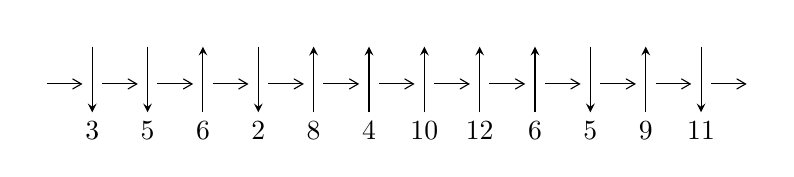
\begin{tikzpicture}[x=20pt, y=17pt]
	% nodes
	\node (C0) at (0, 0) {};
	\node (C1) at (1, 0) {};
	\node (C1U) at (1, +1) {};
	\node (C1D) at (1, -1) {3};

	\node (C2) at (2, 0) {};
	\node (C2U) at (2, +1) {};
	\node (C2D) at (2, -1) {5};

	\node (C3) at (3, 0) {};
	\node (C3U) at (3, +1) {};
	\node (C3D) at (3, -1) {6};

	\node (C4) at (4, 0) {};
	\node (C4U) at (4, +1) {};
	\node (C4D) at (4, -1) {2};

	\node (C5) at (5, 0) {};
	\node (C5U) at (5, +1) {};
	\node (C5D) at (5, -1) {8};

	\node (C6) at (6, 0) {};
	\node (C6U) at (6, +1) {};
	\node (C6D) at (6, -1) {4};

	\node (C7) at (7, 0) {};
	\node (C7U) at (7, +1) {};
	\node (C7D) at (7, -1) {10};

	\node (C8) at (8, 0) {};
	\node (C8U) at (8, +1) {};
	\node (C8D) at (8, -1) {12};

	\node (C9) at (9, 0) {};
	\node (C9U) at (9, +1) {};
	\node (C9D) at (9, -1) {6};

	\node (C10) at (10, 0) {};
	\node (C10U) at (10, +1) {};
	\node (C10D) at (10, -1) {5};

	\node (C11) at (11, 0) {};
	\node (C11U) at (11, +1) {};
	\node (C11D) at (11, -1) {9};

	\node (C12) at (12, 0) {};
	\node (C12U) at (12, +1) {};
	\node (C12D) at (12, -1) {11};
	\node (C13) at (13, 0) {};

	% arrows
	\draw[->,>={angle 60}]
	(C0) edge (C1) (C1) edge (C2) (C2) edge (C3) (C3) edge (C4) (C4) edge (C5) (C5) edge (C6) (C6) edge (C7) (C7) edge (C8) (C8) edge (C9) (C9) edge (C10) (C10) edge (C11) (C11) edge (C12) (C12) edge (C13) ;	\draw[->,>=stealth]
	(C1U) edge (C1D) (C2U) edge (C2D) (C3D) edge (C3U) (C4U) edge (C4D) (C5D) edge (C5U) (C6D) edge (C6U) (C7D) edge (C7U) (C8D) edge (C8U) (C9D) edge (C9U) (C10U) edge (C10D) (C11D) edge (C11U) (C12U) edge (C12D) ;
	\end{tikzpicture} \\
\hhline{~~} \\& 
\textbf{Solving Sequence} \\ \cline{2-2} 
 &
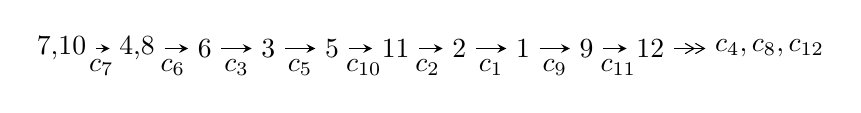
\begin{tikzpicture}[x=23pt, y=7pt]
	% node
	\node (A0) at (-1/8, 0) {7,10};
	\node (A1) at (17/16, 0) {4,8};
	\node (A2) at (17/8, 0) {6};
	\node (A3) at (25/8, 0) {3};
	\node (A4) at (33/8, 0) {5};
	\node (A5) at (41/8, 0) {11};
	\node (A6) at (49/8, 0) {2};
	\node (A7) at (57/8, 0) {1};
	\node (A8) at (65/8, 0) {9};
	\node (A9) at (73/8, 0) {12};
	\node (C1) at (1/2, -1) {$c_{7}$};
	\node (C2) at (13/8, -1) {$c_{6}$};
	\node (C3) at (21/8, -1) {$c_{3}$};
	\node (C4) at (29/8, -1) {$c_{5}$};
	\node (C5) at (37/8, -1) {$c_{10}$};
	\node (C6) at (45/8, -1) {$c_{2}$};
	\node (C7) at (53/8, -1) {$c_{1}$};
	\node (C8) at (61/8, -1) {$c_{9}$};
	\node (C9) at (69/8, -1) {$c_{11}$};
	\node (A10) at (11, 0) {$c_{4},c_{8},c_{12}$};

	% edge
	\draw[->,>=stealth]	
	(A0) edge (A1) (A1) edge (A2) (A2) edge (A3) (A3) edge (A4) (A4) edge (A5) (A5) edge (A6) (A6) edge (A7) (A7) edge (A8) (A8) edge (A9) ;
	\draw[->>,>={angle 60}]	
	(A9) edge (A10);
\end{tikzpicture} \\ 

\end{tabular} \\

\footnotetext{
The image of knot diagram is generated by the software ``\textbf{Draw programme}" developed by Andrew Bartholomew(\url{http://www.layer8.co.uk/maths/draw/index.htm\#Running-draw}), where we modified some parts for our purpose(\url{https://github.com/CATsTAILs/LinksPainter}).
}\phantom \\ \newline 
\centering \textbf{Ideals for irreducible components\footnotemark of $X_{\text{par}}$} 
 
\begin{align*}
I^u_{1}&=\langle 
7.80956\times10^{63} u^{23}-1.02547\times10^{64} u^{22}+\cdots+2.29425\times10^{67} b-5.89286\times10^{67},\\
\phantom{I^u_{1}}&\phantom{= \langle  }1.97576\times10^{64} u^{23}-3.89917\times10^{64} u^{22}+\cdots+4.58851\times10^{67} a-3.71378\times10^{68},\\
\phantom{I^u_{1}}&\phantom{= \langle  }u^{24}-2 u^{23}+\cdots-28672 u+4096\rangle \\
I^u_{2}&=\langle 
b,\;- u^8+2 u^7+2 u^6-5 u^5- u^4+5 u^3- u^2+a,\;u^9- u^8-2 u^7+3 u^6+u^5-3 u^4+2 u^3- u+1\rangle \\
\\
I^v_{1}&=\langle 
a,\;-164522 v^{11}-355934 v^{10}+\cdots+707733 b+176501,\\
\phantom{I^v_{1}}&\phantom{= \langle  }v^{12}+3 v^{11}+3 v^{10}+18 v^9+31 v^8-29 v^7-31 v^6-9 v^5+19 v^4+5 v^3-4 v^2+v+1\rangle \\
\end{align*}
\raggedright * 3 irreducible components of $\dim_{\mathbb{C}}=0$, with total 45 representations.\\
\footnotetext{All coefficients of polynomials are rational numbers. But the coefficients are sometimes approximated in decimal forms when there is not enough margin.}
\newpage
\renewcommand{\arraystretch}{1}
\centering \section*{I. $I^u_{1}= \langle 7.81\times10^{63} u^{23}-1.03\times10^{64} u^{22}+\cdots+2.29\times10^{67} b-5.89\times10^{67},\;1.98\times10^{64} u^{23}-3.90\times10^{64} u^{22}+\cdots+4.59\times10^{67} a-3.71\times10^{68},\;u^{24}-2 u^{23}+\cdots-28672 u+4096 \rangle$}
\flushleft \textbf{(i) Arc colorings}\\
\begin{tabular}{m{7pt} m{180pt} m{7pt} m{180pt} }
\flushright $a_{7}=$&$\begin{pmatrix}1\\0\end{pmatrix}$ \\
\flushright $a_{10}=$&$\begin{pmatrix}0\\u\end{pmatrix}$ \\
\flushright $a_{4}=$&$\begin{pmatrix}-0.000430588 u^{23}+0.000849769 u^{22}+\cdots-30.4322 u+8.09365\\-0.000340396 u^{23}+0.000446971 u^{22}+\cdots-15.0993 u+2.56853\end{pmatrix}$ \\
\flushright $a_{8}=$&$\begin{pmatrix}1\\- u^2\end{pmatrix}$ \\
\flushright $a_{6}=$&$\begin{pmatrix}-0.000770690 u^{23}+0.000886997 u^{22}+\cdots-28.3683 u+4.83639\\0.0000627821 u^{23}-2.14799\times10^{-6} u^{22}+\cdots+0.966055 u-0.729487\end{pmatrix}$ \\
\flushright $a_{3}=$&$\begin{pmatrix}-0.000177123 u^{23}+0.000316023 u^{22}+\cdots-20.9747 u+7.59248\\-0.000440550 u^{23}+0.000737374 u^{22}+\cdots-27.4672 u+4.56426\end{pmatrix}$ \\
\flushright $a_{5}=$&$\begin{pmatrix}-0.000247524 u^{23}+0.000151248 u^{22}+\cdots-13.7287 u+2.88552\\-0.0000743622 u^{23}+0.000208018 u^{22}+\cdots-5.79607 u+0.542658\end{pmatrix}$ \\
\flushright $a_{11}=$&$\begin{pmatrix}0.00108442 u^{23}-0.00207040 u^{22}+\cdots+62.2122 u-10.2669\\0.000158575 u^{23}+0.0000350829 u^{22}+\cdots-7.95177 u+2.38129\end{pmatrix}$ \\
\flushright $a_{2}=$&$\begin{pmatrix}-0.000349715 u^{23}+0.000929736 u^{22}+\cdots-27.5141 u+7.63549\\-0.000471953 u^{23}+0.000545981 u^{22}+\cdots-19.0997 u+3.40520\end{pmatrix}$ \\
\flushright $a_{1}=$&$\begin{pmatrix}-0.000974598 u^{23}+0.00198880 u^{22}+\cdots-59.8532 u+10.2543\\-0.000406712 u^{23}+0.000387216 u^{22}+\cdots-5.12759 u+0.162234\end{pmatrix}$ \\
\flushright $a_{9}=$&$\begin{pmatrix}0.00105057 u^{23}-0.00167229 u^{22}+\cdots+45.4181 u-7.13094\\-0.000133803 u^{23}+0.000328867 u^{22}+\cdots-13.2158 u+2.91448\end{pmatrix}$ \\
\flushright $a_{12}=$&$\begin{pmatrix}0.00207530 u^{23}-0.00334512 u^{22}+\cdots+88.7435 u-14.5857\\0.000298832 u^{23}-0.0000705567 u^{22}+\cdots-4.27903 u+1.62940\end{pmatrix}$\\&\end{tabular}
\flushleft \textbf{(ii) Obstruction class $= -1$}\\~\\
\flushleft \textbf{(iii) Cusp Shapes $= -0.000912531 u^{23}+0.00194308 u^{22}+\cdots-44.5011 u+4.80932$}\\~\\
\newpage\renewcommand{\arraystretch}{1}
\flushleft \textbf{(iv) u-Polynomials at the component}\newline \\
\begin{tabular}{m{50pt}|m{274pt}}
Crossings & \hspace{64pt}u-Polynomials at each crossing \\
\hline $$\begin{aligned}c_{1}\end{aligned}$$&$\begin{aligned}
&u^{24}+24 u^{23}+\cdots-179 u+1
\end{aligned}$\\
\hline $$\begin{aligned}c_{2},c_{4}\end{aligned}$$&$\begin{aligned}
&u^{24}-12 u^{23}+\cdots+17 u-1
\end{aligned}$\\
\hline $$\begin{aligned}c_{3},c_{6}\end{aligned}$$&$\begin{aligned}
&u^{24}+u^{23}+\cdots-2560 u+512
\end{aligned}$\\
\hline $$\begin{aligned}c_{5}\end{aligned}$$&$\begin{aligned}
&u^{24}+4 u^{23}+\cdots-3 u-1
\end{aligned}$\\
\hline $$\begin{aligned}c_{7}\end{aligned}$$&$\begin{aligned}
&u^{24}+2 u^{23}+\cdots+28672 u+4096
\end{aligned}$\\
\hline $$\begin{aligned}c_{8},c_{11}\end{aligned}$$&$\begin{aligned}
&u^{24}+8 u^{23}+\cdots+7 u+1
\end{aligned}$\\
\hline $$\begin{aligned}c_{9}\end{aligned}$$&$\begin{aligned}
&u^{24}+u^{23}+\cdots-74162 u-19441
\end{aligned}$\\
\hline $$\begin{aligned}c_{10}\end{aligned}$$&$\begin{aligned}
&u^{24}-5 u^{23}+\cdots-389242 u+249139
\end{aligned}$\\
\hline $$\begin{aligned}c_{12}\end{aligned}$$&$\begin{aligned}
&u^{24}+20 u^{22}+\cdots+19 u+1
\end{aligned}$\\
\hline
\end{tabular}\\~\\
\newpage\renewcommand{\arraystretch}{1}
\flushleft \textbf{(v) Riley Polynomials at the component}\newline \\
\begin{tabular}{m{50pt}|m{274pt}}
Crossings & \hspace{64pt}Riley Polynomials at each crossing \\
\hline $$\begin{aligned}c_{1}\end{aligned}$$&$\begin{aligned}
&y^{24}+204 y^{23}+\cdots-2901 y+1
\end{aligned}$\\
\hline $$\begin{aligned}c_{2},c_{4}\end{aligned}$$&$\begin{aligned}
&y^{24}-24 y^{23}+\cdots+179 y+1
\end{aligned}$\\
\hline $$\begin{aligned}c_{3},c_{6}\end{aligned}$$&$\begin{aligned}
&y^{24}-63 y^{23}+\cdots-3932160 y+262144
\end{aligned}$\\
\hline $$\begin{aligned}c_{5}\end{aligned}$$&$\begin{aligned}
&y^{24}+26 y^{22}+\cdots- y+1
\end{aligned}$\\
\hline $$\begin{aligned}c_{7}\end{aligned}$$&$\begin{aligned}
&y^{24}-90 y^{23}+\cdots+67108864 y+16777216
\end{aligned}$\\
\hline $$\begin{aligned}c_{8},c_{11}\end{aligned}$$&$\begin{aligned}
&y^{24}+20 y^{22}+\cdots+19 y+1
\end{aligned}$\\
\hline $$\begin{aligned}c_{9}\end{aligned}$$&$\begin{aligned}
&y^{24}-61 y^{23}+\cdots-296113128 y+377952481
\end{aligned}$\\
\hline $$\begin{aligned}c_{10}\end{aligned}$$&$\begin{aligned}
&y^{24}+111 y^{23}+\cdots-469614992544 y+62070241321
\end{aligned}$\\
\hline $$\begin{aligned}c_{12}\end{aligned}$$&$\begin{aligned}
&y^{24}+40 y^{23}+\cdots+2151 y+1
\end{aligned}$\\
\hline
\end{tabular}\\~\\
\newpage\flushleft \textbf{(vi) Complex Volumes and Cusp Shapes}
$$\begin{array}{c|c|c}  
\text{Solutions to }I^u_{1}& \I (\text{vol} + \sqrt{-1}CS) & \text{Cusp shape}\\
 \hline 
\begin{aligned}
u &= -0.632443 + 0.726844 I \\
a &= \phantom{-}0.114777 + 0.151496 I \\
b &= \phantom{-}1.063560 + 0.162285 I\end{aligned}
 & \phantom{-}2.67249 - 0.06243 I & \phantom{-}6.49122 - 0.13400 I \\ \hline\begin{aligned}
u &= -0.632443 - 0.726844 I \\
a &= \phantom{-}0.114777 - 0.151496 I \\
b &= \phantom{-}1.063560 - 0.162285 I\end{aligned}
 & \phantom{-}2.67249 + 0.06243 I & \phantom{-}6.49122 + 0.13400 I \\ \hline\begin{aligned}
u &= \phantom{-}1.201550 + 0.153048 I \\
a &= \phantom{-}0.0923620 + 0.0946298 I \\
b &= -0.828567 + 0.942729 I\end{aligned}
 & \phantom{-}1.03909 - 7.66938 I & \phantom{-}3.58752 + 6.84907 I \\ \hline\begin{aligned}
u &= \phantom{-}1.201550 - 0.153048 I \\
a &= \phantom{-}0.0923620 - 0.0946298 I \\
b &= -0.828567 - 0.942729 I\end{aligned}
 & \phantom{-}1.03909 + 7.66938 I & \phantom{-}3.58752 - 6.84907 I \\ \hline\begin{aligned}
u &= \phantom{-}0.690057 + 0.202830 I \\
a &= \phantom{-}2.59655 - 0.30553 I \\
b &= -0.024221 - 0.599362 I\end{aligned}
 & -1.38798 - 2.82419 I & \phantom{-}0.59813 + 2.55909 I \\ \hline\begin{aligned}
u &= \phantom{-}0.690057 - 0.202830 I \\
a &= \phantom{-}2.59655 + 0.30553 I \\
b &= -0.024221 + 0.599362 I\end{aligned}
 & -1.38798 + 2.82419 I & \phantom{-}0.59813 - 2.55909 I \\ \hline\begin{aligned}
u &= \phantom{-}0.505730 + 0.448375 I \\
a &= \phantom{-}2.58887 - 1.75795 I \\
b &= -0.950717 + 0.074911 I\end{aligned}
 & -2.60567 + 1.37963 I & -1.96914 - 4.05392 I \\ \hline\begin{aligned}
u &= \phantom{-}0.505730 - 0.448375 I \\
a &= \phantom{-}2.58887 + 1.75795 I \\
b &= -0.950717 - 0.074911 I\end{aligned}
 & -2.60567 - 1.37963 I & -1.96914 + 4.05392 I \\ \hline\begin{aligned}
u &= -0.661121\phantom{ +0.000000I} \\
a &= \phantom{-}0.510618\phantom{ +0.000000I} \\
b &= \phantom{-}0.373534\phantom{ +0.000000I}\end{aligned}
 & \phantom{-}1.02845\phantom{ +0.000000I} & \phantom{-}10.2860\phantom{ +0.000000I} \\ \hline\begin{aligned}
u &= \phantom{-}0.049304 + 0.644470 I \\
a &= \phantom{-}1.84071 - 0.43802 I \\
b &= \phantom{-}0.232697 - 0.155126 I\end{aligned}
 & \phantom{-}0.59509 - 2.36713 I & \phantom{-}1.40991 + 3.67925 I\\
 \hline 
 \end{array}$$\newpage$$\begin{array}{c|c|c}  
\text{Solutions to }I^u_{1}& \I (\text{vol} + \sqrt{-1}CS) & \text{Cusp shape}\\
 \hline 
\begin{aligned}
u &= \phantom{-}0.049304 - 0.644470 I \\
a &= \phantom{-}1.84071 + 0.43802 I \\
b &= \phantom{-}0.232697 + 0.155126 I\end{aligned}
 & \phantom{-}0.59509 + 2.36713 I & \phantom{-}1.40991 - 3.67925 I \\ \hline\begin{aligned}
u &= \phantom{-}1.17039 + 0.90470 I \\
a &= \phantom{-}0.319512 - 0.046660 I \\
b &= -0.893023 + 0.472118 I\end{aligned}
 & -1.87950 + 2.72151 I & \phantom{-}1.13774 - 4.25269 I \\ \hline\begin{aligned}
u &= \phantom{-}1.17039 - 0.90470 I \\
a &= \phantom{-}0.319512 + 0.046660 I \\
b &= -0.893023 - 0.472118 I\end{aligned}
 & -1.87950 - 2.72151 I & \phantom{-}1.13774 + 4.25269 I \\ \hline\begin{aligned}
u &= \phantom{-}0.188201 + 0.357668 I \\
a &= \phantom{-}2.01717 - 1.17792 I \\
b &= -0.349958 - 0.812535 I\end{aligned}
 & -1.83062 - 1.07717 I & -2.53581 + 1.58170 I \\ \hline\begin{aligned}
u &= \phantom{-}0.188201 - 0.357668 I \\
a &= \phantom{-}2.01717 + 1.17792 I \\
b &= -0.349958 + 0.812535 I\end{aligned}
 & -1.83062 + 1.07717 I & -2.53581 - 1.58170 I \\ \hline\begin{aligned}
u &= -2.38858 + 1.57335 I \\
a &= -0.524904 - 0.425161 I \\
b &= \phantom{-}2.09180 - 1.57981 I\end{aligned}
 & \phantom{-}18.8685 - 6.6483 I & \phantom{-0.000000 } 0 \\ \hline\begin{aligned}
u &= -2.38858 - 1.57335 I \\
a &= -0.524904 + 0.425161 I \\
b &= \phantom{-}2.09180 + 1.57981 I\end{aligned}
 & \phantom{-}18.8685 + 6.6483 I & \phantom{-0.000000 } 0 \\ \hline\begin{aligned}
u &= \phantom{-}2.25638 + 1.80466 I \\
a &= \phantom{-}0.568423 - 0.488334 I \\
b &= -2.24002 - 1.53390 I\end{aligned}
 & \phantom{-}18.7357 + 14.2573 I & \phantom{-0.000000 } 0 \\ \hline\begin{aligned}
u &= \phantom{-}2.25638 - 1.80466 I \\
a &= \phantom{-}0.568423 + 0.488334 I \\
b &= -2.24002 + 1.53390 I\end{aligned}
 & \phantom{-}18.7357 - 14.2573 I & \phantom{-0.000000 } 0 \\ \hline\begin{aligned}
u &= -3.61633\phantom{ +0.000000I} \\
a &= -0.660672\phantom{ +0.000000I} \\
b &= \phantom{-}2.14769\phantom{ +0.000000I}\end{aligned}
 & \phantom{-}0.756608\phantom{ +0.000000I} & \phantom{-0.000000 } 0\\
 \hline 
 \end{array}$$\newpage$$\begin{array}{c|c|c}  
\text{Solutions to }I^u_{1}& \I (\text{vol} + \sqrt{-1}CS) & \text{Cusp shape}\\
 \hline 
\begin{aligned}
u &= \phantom{-}4.44102 + 1.22807 I \\
a &= -0.408012 + 0.133656 I \\
b &= \phantom{-}3.93681 + 1.85539 I\end{aligned}
 & -18.9745 - 1.9748 I & \phantom{-0.000000 } 0 \\ \hline\begin{aligned}
u &= \phantom{-}4.44102 - 1.22807 I \\
a &= -0.408012 - 0.133656 I \\
b &= \phantom{-}3.93681 - 1.85539 I\end{aligned}
 & -18.9745 + 1.9748 I & \phantom{-0.000000 } 0 \\ \hline\begin{aligned}
u &= -4.34288 + 2.39260 I \\
a &= \phantom{-}0.369569 + 0.203301 I \\
b &= -3.79897 + 1.84880 I\end{aligned}
 & -18.5925 - 5.6388 I & \phantom{-0.000000 } 0 \\ \hline\begin{aligned}
u &= -4.34288 - 2.39260 I \\
a &= \phantom{-}0.369569 - 0.203301 I \\
b &= -3.79897 - 1.84880 I\end{aligned}
 & -18.5925 + 5.6388 I & \phantom{-0.000000 } 0\\
 \hline 
 \end{array}$$\newpage\newpage\renewcommand{\arraystretch}{1}
\centering \section*{II. $I^u_{2}= \langle b,\;- u^8+2 u^7+2 u^6-5 u^5- u^4+5 u^3- u^2+a,\;u^9- u^8-2 u^7+3 u^6+u^5-3 u^4+2 u^3- u+1 \rangle$}
\flushleft \textbf{(i) Arc colorings}\\
\begin{tabular}{m{7pt} m{180pt} m{7pt} m{180pt} }
\flushright $a_{7}=$&$\begin{pmatrix}1\\0\end{pmatrix}$ \\
\flushright $a_{10}=$&$\begin{pmatrix}0\\u\end{pmatrix}$ \\
\flushright $a_{4}=$&$\begin{pmatrix}u^8-2 u^7-2 u^6+5 u^5+u^4-5 u^3+u^2\\0\end{pmatrix}$ \\
\flushright $a_{8}=$&$\begin{pmatrix}1\\- u^2\end{pmatrix}$ \\
\flushright $a_{6}=$&$\begin{pmatrix}1\\0\end{pmatrix}$ \\
\flushright $a_{3}=$&$\begin{pmatrix}u^8-2 u^7-2 u^6+5 u^5+u^4-5 u^3+u^2\\0\end{pmatrix}$ \\
\flushright $a_{5}=$&$\begin{pmatrix}- u^2+1\\u^4\end{pmatrix}$ \\
\flushright $a_{11}=$&$\begin{pmatrix}- u^5+2 u^3- u\\u^7- u^5+u\end{pmatrix}$ \\
\flushright $a_{2}=$&$\begin{pmatrix}u^8-2 u^7-2 u^6+5 u^5+u^4-5 u^3+2 u^2-1\\- u^4\end{pmatrix}$ \\
\flushright $a_{1}=$&$\begin{pmatrix}u^2-1\\- u^4\end{pmatrix}$ \\
\flushright $a_{9}=$&$\begin{pmatrix}- u\\u\end{pmatrix}$ \\
\flushright $a_{12}=$&$\begin{pmatrix}u^8-3 u^6+3 u^4-1\\- u^8+u^7+3 u^6-2 u^5-3 u^4+2 u^3+1\end{pmatrix}$\\&\end{tabular}
\flushleft \textbf{(ii) Obstruction class $= 1$}\\~\\
\flushleft \textbf{(iii) Cusp Shapes $= -5 u^8+u^7+7 u^6-6 u^5-6 u^4+7 u^3-5 u^2-7 u+1$}\\~\\
\newpage\renewcommand{\arraystretch}{1}
\flushleft \textbf{(iv) u-Polynomials at the component}\newline \\
\begin{tabular}{m{50pt}|m{274pt}}
Crossings & \hspace{64pt}u-Polynomials at each crossing \\
\hline $$\begin{aligned}c_{1},c_{2}\end{aligned}$$&$\begin{aligned}
&(u-1)^9
\end{aligned}$\\
\hline $$\begin{aligned}c_{3},c_{6}\end{aligned}$$&$\begin{aligned}
&u^9
\end{aligned}$\\
\hline $$\begin{aligned}c_{4}\end{aligned}$$&$\begin{aligned}
&(u+1)^9
\end{aligned}$\\
\hline $$\begin{aligned}c_{5}\end{aligned}$$&$\begin{aligned}
&u^9+5 u^8+12 u^7+15 u^6+9 u^5- u^4-4 u^3-2 u^2+u+1
\end{aligned}$\\
\hline $$\begin{aligned}c_{7}\end{aligned}$$&$\begin{aligned}
&u^9- u^8-2 u^7+3 u^6+u^5-3 u^4+2 u^3- u+1
\end{aligned}$\\
\hline $$\begin{aligned}c_{8}\end{aligned}$$&$\begin{aligned}
&u^9- u^8+2 u^7- u^6+3 u^5- u^4+2 u^3+u+1
\end{aligned}$\\
\hline $$\begin{aligned}c_{9}\end{aligned}$$&$\begin{aligned}
&u^9+u^8-2 u^7-3 u^6+u^5+3 u^4+2 u^3- u-1
\end{aligned}$\\
\hline $$\begin{aligned}c_{10},c_{12}\end{aligned}$$&$\begin{aligned}
&u^9+3 u^8+8 u^7+13 u^6+17 u^5+17 u^4+12 u^3+6 u^2+u-1
\end{aligned}$\\
\hline $$\begin{aligned}c_{11}\end{aligned}$$&$\begin{aligned}
&u^9+u^8+2 u^7+u^6+3 u^5+u^4+2 u^3+u-1
\end{aligned}$\\
\hline
\end{tabular}\\~\\
\newpage\renewcommand{\arraystretch}{1}
\flushleft \textbf{(v) Riley Polynomials at the component}\newline \\
\begin{tabular}{m{50pt}|m{274pt}}
Crossings & \hspace{64pt}Riley Polynomials at each crossing \\
\hline $$\begin{aligned}c_{1},c_{2},c_{4}\end{aligned}$$&$\begin{aligned}
&(y-1)^9
\end{aligned}$\\
\hline $$\begin{aligned}c_{3},c_{6}\end{aligned}$$&$\begin{aligned}
&y^9
\end{aligned}$\\
\hline $$\begin{aligned}c_{5}\end{aligned}$$&$\begin{aligned}
&y^9- y^8+12 y^7-7 y^6+37 y^5+y^4-10 y^2+5 y-1
\end{aligned}$\\
\hline $$\begin{aligned}c_{7},c_{9}\end{aligned}$$&$\begin{aligned}
&y^9-5 y^8+12 y^7-15 y^6+9 y^5+y^4-4 y^3+2 y^2+y-1
\end{aligned}$\\
\hline $$\begin{aligned}c_{8},c_{11}\end{aligned}$$&$\begin{aligned}
&y^9+3 y^8+8 y^7+13 y^6+17 y^5+17 y^4+12 y^3+6 y^2+y-1
\end{aligned}$\\
\hline $$\begin{aligned}c_{10},c_{12}\end{aligned}$$&$\begin{aligned}
&y^9+7 y^8+20 y^7+25 y^6+5 y^5-15 y^4+22 y^2+13 y-1
\end{aligned}$\\
\hline
\end{tabular}\\~\\
\newpage\flushleft \textbf{(vi) Complex Volumes and Cusp Shapes}
$$\begin{array}{c|c|c}  
\text{Solutions to }I^u_{2}& \I (\text{vol} + \sqrt{-1}CS) & \text{Cusp shape}\\
 \hline 
\begin{aligned}
u &= \phantom{-}0.772920 + 0.510351 I \\
a &= -0.939568 - 0.981640 I \\
b &= \phantom{-0.000000 } 0\end{aligned}
 & -3.42837 + 2.09337 I & -4.41045 - 5.46639 I \\ \hline\begin{aligned}
u &= \phantom{-}0.772920 - 0.510351 I \\
a &= -0.939568 + 0.981640 I \\
b &= \phantom{-0.000000 } 0\end{aligned}
 & -3.42837 - 2.09337 I & -4.41045 + 5.46639 I \\ \hline\begin{aligned}
u &= -0.825933\phantom{ +0.000000I} \\
a &= \phantom{-}2.14893\phantom{ +0.000000I} \\
b &= \phantom{-0.000000 } 0\end{aligned}
 & -0.446489\phantom{ +0.000000I} & -0.182090\phantom{ +0.000000I} \\ \hline\begin{aligned}
u &= -1.173910 + 0.391555 I \\
a &= \phantom{-}0.119081 + 0.409451 I \\
b &= \phantom{-0.000000 } 0\end{aligned}
 & \phantom{-}2.72642 - 1.33617 I & \phantom{-}8.07941 + 3.55369 I \\ \hline\begin{aligned}
u &= -1.173910 - 0.391555 I \\
a &= \phantom{-}0.119081 - 0.409451 I \\
b &= \phantom{-0.000000 } 0\end{aligned}
 & \phantom{-}2.72642 + 1.33617 I & \phantom{-}8.07941 - 3.55369 I \\ \hline\begin{aligned}
u &= \phantom{-}0.141484 + 0.739668 I \\
a &= \phantom{-}2.26219 + 2.13290 I \\
b &= \phantom{-0.000000 } 0\end{aligned}
 & -1.02799 - 2.45442 I & -2.24638 - 6.63381 I \\ \hline\begin{aligned}
u &= \phantom{-}0.141484 - 0.739668 I \\
a &= \phantom{-}2.26219 - 2.13290 I \\
b &= \phantom{-0.000000 } 0\end{aligned}
 & -1.02799 + 2.45442 I & -2.24638 + 6.63381 I \\ \hline\begin{aligned}
u &= \phantom{-}1.172470 + 0.500383 I \\
a &= -0.016164 - 0.378317 I \\
b &= \phantom{-0.000000 } 0\end{aligned}
 & \phantom{-}1.95319 + 7.08493 I & \phantom{-}8.66846 - 5.33071 I \\ \hline\begin{aligned}
u &= \phantom{-}1.172470 - 0.500383 I \\
a &= -0.016164 + 0.378317 I \\
b &= \phantom{-0.000000 } 0\end{aligned}
 & \phantom{-}1.95319 - 7.08493 I & \phantom{-}8.66846 + 5.33071 I\\
 \hline 
 \end{array}$$\newpage\newpage\renewcommand{\arraystretch}{1}
\centering \section*{III. $I^v_{1}= \langle a,\;-1.65\times10^{5} v^{11}-3.56\times10^{5} v^{10}+\cdots+7.08\times10^{5} b+1.77\times10^{5},\;v^{12}+3 v^{11}+\cdots+v+1 \rangle$}
\flushleft \textbf{(i) Arc colorings}\\
\begin{tabular}{m{7pt} m{180pt} m{7pt} m{180pt} }
\flushright $a_{7}=$&$\begin{pmatrix}1\\0\end{pmatrix}$ \\
\flushright $a_{10}=$&$\begin{pmatrix}v\\0\end{pmatrix}$ \\
\flushright $a_{4}=$&$\begin{pmatrix}0\\0.232463 v^{11}+0.502921 v^{10}+\cdots-0.152902 v-0.249389\end{pmatrix}$ \\
\flushright $a_{8}=$&$\begin{pmatrix}1\\0\end{pmatrix}$ \\
\flushright $a_{6}=$&$\begin{pmatrix}1\\-1.04198 v^{11}-2.90360 v^{10}+\cdots+1.23849 v-0.574544\end{pmatrix}$ \\
\flushright $a_{3}=$&$\begin{pmatrix}-0.232463 v^{11}-0.502921 v^{10}+\cdots+0.152902 v+0.249389\\-1.00827 v^{11}-2.68986 v^{10}+\cdots+1.09637 v-2.28028\end{pmatrix}$ \\
\flushright $a_{5}=$&$\begin{pmatrix}1.04198 v^{11}+2.90360 v^{10}+\cdots-1.23849 v+1.57454\\-1.04198 v^{11}-2.90360 v^{10}+\cdots+1.23849 v-0.574544\end{pmatrix}$ \\
\flushright $a_{11}=$&$\begin{pmatrix}-0.126775 v^{11}-0.205966 v^{10}+\cdots+2.64946 v-0.819476\\0.349127 v^{11}+0.655942 v^{10}+\cdots-1.18202 v+1.86146\end{pmatrix}$ \\
\flushright $a_{2}=$&$\begin{pmatrix}0.819476 v^{11}+2.33165 v^{10}+\cdots-1.01499 v+1.46894\\-1.62222 v^{11}-4.40786 v^{10}+\cdots+1.83221 v-1.73501\end{pmatrix}$ \\
\flushright $a_{1}=$&$\begin{pmatrix}-1\\0\end{pmatrix}$ \\
\flushright $a_{9}=$&$\begin{pmatrix}0.222352 v^{11}+0.449976 v^{10}+\cdots+1.46744 v+1.04198\\0.349127 v^{11}+0.655942 v^{10}+\cdots-1.18202 v+1.86146\end{pmatrix}$ \\
\flushright $a_{12}=$&$\begin{pmatrix}-0.989917 v^{11}-2.68233 v^{10}+\cdots+3.73598 v-2.22768\\0.349127 v^{11}+0.655942 v^{10}+\cdots-1.18202 v+0.861460\end{pmatrix}$\\&\end{tabular}
\flushleft \textbf{(ii) Obstruction class $= 1$}\\~\\
\flushleft \textbf{(iii) Cusp Shapes $= \frac{1086197}{235911} v^{11}+\frac{2821982}{235911} v^{10}+\cdots-\frac{94285}{235911} v+\frac{2199643}{235911}$}\\~\\
\newpage\renewcommand{\arraystretch}{1}
\flushleft \textbf{(iv) u-Polynomials at the component}\newline \\
\begin{tabular}{m{50pt}|m{274pt}}
Crossings & \hspace{64pt}u-Polynomials at each crossing \\
\hline $$\begin{aligned}c_{1}\end{aligned}$$&$\begin{aligned}
&(u^6-3 u^5+5 u^4-4 u^3+2 u^2- u+1)^2
\end{aligned}$\\
\hline $$\begin{aligned}c_{2},c_{6}\end{aligned}$$&$\begin{aligned}
&(u^6+u^5- u^4-2 u^3+u+1)^2
\end{aligned}$\\
\hline $$\begin{aligned}c_{3},c_{4}\end{aligned}$$&$\begin{aligned}
&(u^6- u^5- u^4+2 u^3- u+1)^2
\end{aligned}$\\
\hline $$\begin{aligned}c_{5}\end{aligned}$$&$\begin{aligned}
&(u^6+3 u^5+5 u^4+4 u^3+2 u^2+u+1)^2
\end{aligned}$\\
\hline $$\begin{aligned}c_{7}\end{aligned}$$&$\begin{aligned}
&u^{12}
\end{aligned}$\\
\hline $$\begin{aligned}c_{8},c_{12}\end{aligned}$$&$\begin{aligned}
&(u^2+u+1)^6
\end{aligned}$\\
\hline $$\begin{aligned}c_{9},c_{10}\end{aligned}$$&$\begin{aligned}
&u^{12}- u^{11}+\cdots-3 u+1
\end{aligned}$\\
\hline $$\begin{aligned}c_{11}\end{aligned}$$&$\begin{aligned}
&(u^2- u+1)^6
\end{aligned}$\\
\hline
\end{tabular}\\~\\
\newpage\renewcommand{\arraystretch}{1}
\flushleft \textbf{(v) Riley Polynomials at the component}\newline \\
\begin{tabular}{m{50pt}|m{274pt}}
Crossings & \hspace{64pt}Riley Polynomials at each crossing \\
\hline $$\begin{aligned}c_{1},c_{5}\end{aligned}$$&$\begin{aligned}
&(y^6+y^5+5 y^4+6 y^2+3 y+1)^2
\end{aligned}$\\
\hline $$\begin{aligned}c_{2},c_{3},c_{4}\\c_{6}\end{aligned}$$&$\begin{aligned}
&(y^6-3 y^5+5 y^4-4 y^3+2 y^2- y+1)^2
\end{aligned}$\\
\hline $$\begin{aligned}c_{7}\end{aligned}$$&$\begin{aligned}
&y^{12}
\end{aligned}$\\
\hline $$\begin{aligned}c_{8},c_{11},c_{12}\end{aligned}$$&$\begin{aligned}
&(y^2+y+1)^6
\end{aligned}$\\
\hline $$\begin{aligned}c_{9},c_{10}\end{aligned}$$&$\begin{aligned}
&y^{12}-3 y^{11}+\cdots- y+1
\end{aligned}$\\
\hline
\end{tabular}\\~\\
\newpage\flushleft \textbf{(vi) Complex Volumes and Cusp Shapes}
$$\begin{array}{c|c|c}  
\text{Solutions to }I^v_{1}& \I (\text{vol} + \sqrt{-1}CS) & \text{Cusp shape}\\
 \hline 
\begin{aligned}
v &= \phantom{-}0.834826 + 0.083652 I \\
a &= \phantom{-0.000000 } 0 \\
b &= \phantom{-}1.002190 - 0.295542 I\end{aligned}
 & \phantom{-}1.89061 + 1.10558 I & \phantom{-}3.63443 - 2.52768 I \\ \hline\begin{aligned}
v &= \phantom{-}0.834826 - 0.083652 I \\
a &= \phantom{-0.000000 } 0 \\
b &= \phantom{-}1.002190 + 0.295542 I\end{aligned}
 & \phantom{-}1.89061 - 1.10558 I & \phantom{-}3.63443 + 2.52768 I \\ \hline\begin{aligned}
v &= -0.489858 + 0.681154 I \\
a &= \phantom{-0.000000 } 0 \\
b &= \phantom{-}1.002190 - 0.295542 I\end{aligned}
 & \phantom{-}1.89061 - 2.95419 I & \phantom{-}6.39280 + 3.57892 I \\ \hline\begin{aligned}
v &= -0.489858 - 0.681154 I \\
a &= \phantom{-0.000000 } 0 \\
b &= \phantom{-}1.002190 + 0.295542 I\end{aligned}
 & \phantom{-}1.89061 + 2.95419 I & \phantom{-}6.39280 - 3.57892 I \\ \hline\begin{aligned}
v &= -0.458424 + 0.081263 I \\
a &= \phantom{-0.000000 } 0 \\
b &= -1.073950 + 0.558752 I\end{aligned}
 & \phantom{-0.000000 } -7.72290 I & -2.53591 + 7.46338 I \\ \hline\begin{aligned}
v &= -0.458424 - 0.081263 I \\
a &= \phantom{-0.000000 } 0 \\
b &= -1.073950 - 0.558752 I\end{aligned}
 & \phantom{-0.000000 -}7.72290 I & -2.53591 - 7.46338 I \\ \hline\begin{aligned}
v &= \phantom{-}0.299588 + 0.356375 I \\
a &= \phantom{-0.000000 } 0 \\
b &= -1.073950 + 0.558752 I\end{aligned}
 & \phantom{-0.000000 } -3.66314 I & \phantom{-}2.83009 + 6.37777 I \\ \hline\begin{aligned}
v &= \phantom{-}0.299588 - 0.356375 I \\
a &= \phantom{-0.000000 } 0 \\
b &= -1.073950 - 0.558752 I\end{aligned}
 & \phantom{-0.000000 -}3.66314 I & \phantom{-}2.83009 - 6.37777 I \\ \hline\begin{aligned}
v &= -2.51133 + 0.49706 I \\
a &= \phantom{-0.000000 } 0 \\
b &= -0.428243 + 0.664531 I\end{aligned}
 & -1.89061 + 2.95419 I & -7.91752 - 1.81989 I \\ \hline\begin{aligned}
v &= -2.51133 - 0.49706 I \\
a &= \phantom{-0.000000 } 0 \\
b &= -0.428243 - 0.664531 I\end{aligned}
 & -1.89061 - 2.95419 I & -7.91752 + 1.81989 I\\
 \hline 
 \end{array}$$\newpage$$\begin{array}{c|c|c}  
\text{Solutions to }I^v_{1}& \I (\text{vol} + \sqrt{-1}CS) & \text{Cusp shape}\\
 \hline 
\begin{aligned}
v &= \phantom{-}0.82520 + 2.42341 I \\
a &= \phantom{-0.000000 } 0 \\
b &= -0.428243 - 0.664531 I\end{aligned}
 & -1.89061 + 1.10558 I & \phantom{-}3.59610 - 6.57635 I \\ \hline\begin{aligned}
v &= \phantom{-}0.82520 - 2.42341 I \\
a &= \phantom{-0.000000 } 0 \\
b &= -0.428243 + 0.664531 I\end{aligned}
 & -1.89061 - 1.10558 I & \phantom{-}3.59610 + 6.57635 I\\
 \hline 
 \end{array}$$\newpage
\newpage\renewcommand{\arraystretch}{1}
\centering \section*{ IV. u-Polynomials}
\begin{tabular}{m{50pt}|m{274pt}}
Crossings & \hspace{64pt}u-Polynomials at each crossing \\
\hline $$\begin{aligned}c_{1}\end{aligned}$$&$\begin{aligned}
&(u-1)^9(u^6-3 u^5+5 u^4-4 u^3+2 u^2- u+1)^2\\
&\cdot(u^{24}+24 u^{23}+\cdots-179 u+1)
\end{aligned}$\\
\hline $$\begin{aligned}c_{2}\end{aligned}$$&$\begin{aligned}
&((u-1)^9)(u^6+u^5+\cdots+u+1)^{2}(u^{24}-12 u^{23}+\cdots+17 u-1)
\end{aligned}$\\
\hline $$\begin{aligned}c_{3}\end{aligned}$$&$\begin{aligned}
&u^9(u^6- u^5+\cdots- u+1)^{2}(u^{24}+u^{23}+\cdots-2560 u+512)
\end{aligned}$\\
\hline $$\begin{aligned}c_{4}\end{aligned}$$&$\begin{aligned}
&((u+1)^9)(u^6- u^5+\cdots- u+1)^{2}(u^{24}-12 u^{23}+\cdots+17 u-1)
\end{aligned}$\\
\hline $$\begin{aligned}c_{5}\end{aligned}$$&$\begin{aligned}
&(u^6+3 u^5+5 u^4+4 u^3+2 u^2+u+1)^2\\
&\cdot(u^9+5 u^8+12 u^7+15 u^6+9 u^5- u^4-4 u^3-2 u^2+u+1)\\
&\cdot(u^{24}+4 u^{23}+\cdots-3 u-1)
\end{aligned}$\\
\hline $$\begin{aligned}c_{6}\end{aligned}$$&$\begin{aligned}
&u^9(u^6+u^5+\cdots+u+1)^{2}(u^{24}+u^{23}+\cdots-2560 u+512)
\end{aligned}$\\
\hline $$\begin{aligned}c_{7}\end{aligned}$$&$\begin{aligned}
&u^{12}(u^9- u^8-2 u^7+3 u^6+u^5-3 u^4+2 u^3- u+1)\\
&\cdot(u^{24}+2 u^{23}+\cdots+28672 u+4096)
\end{aligned}$\\
\hline $$\begin{aligned}c_{8}\end{aligned}$$&$\begin{aligned}
&(u^2+u+1)^6(u^9- u^8+2 u^7- u^6+3 u^5- u^4+2 u^3+u+1)\\
&\cdot(u^{24}+8 u^{23}+\cdots+7 u+1)
\end{aligned}$\\
\hline $$\begin{aligned}c_{9}\end{aligned}$$&$\begin{aligned}
&(u^9+u^8+\cdots- u-1)(u^{12}- u^{11}+\cdots-3 u+1)\\
&\cdot(u^{24}+u^{23}+\cdots-74162 u-19441)
\end{aligned}$\\
\hline $$\begin{aligned}c_{10}\end{aligned}$$&$\begin{aligned}
&(u^9+3 u^8+8 u^7+13 u^6+17 u^5+17 u^4+12 u^3+6 u^2+u-1)\\
&\cdot(u^{12}- u^{11}+\cdots-3 u+1)(u^{24}-5 u^{23}+\cdots-389242 u+249139)
\end{aligned}$\\
\hline $$\begin{aligned}c_{11}\end{aligned}$$&$\begin{aligned}
&(u^2- u+1)^6(u^9+u^8+2 u^7+u^6+3 u^5+u^4+2 u^3+u-1)\\
&\cdot(u^{24}+8 u^{23}+\cdots+7 u+1)
\end{aligned}$\\
\hline $$\begin{aligned}c_{12}\end{aligned}$$&$\begin{aligned}
&(u^2+u+1)^6\\
&\cdot(u^9+3 u^8+8 u^7+13 u^6+17 u^5+17 u^4+12 u^3+6 u^2+u-1)\\
&\cdot(u^{24}+20 u^{22}+\cdots+19 u+1)
\end{aligned}$\\
\hline
\end{tabular}\newpage\renewcommand{\arraystretch}{1}
\centering \section*{ V. Riley Polynomials}
\begin{tabular}{m{50pt}|m{274pt}}
Crossings & \hspace{64pt}Riley Polynomials at each crossing \\
\hline $$\begin{aligned}c_{1}\end{aligned}$$&$\begin{aligned}
&(y-1)^9(y^6+y^5+5 y^4+6 y^2+3 y+1)^2\\
&\cdot(y^{24}+204 y^{23}+\cdots-2901 y+1)
\end{aligned}$\\
\hline $$\begin{aligned}c_{2},c_{4}\end{aligned}$$&$\begin{aligned}
&(y-1)^9(y^6-3 y^5+5 y^4-4 y^3+2 y^2- y+1)^2\\
&\cdot(y^{24}-24 y^{23}+\cdots+179 y+1)
\end{aligned}$\\
\hline $$\begin{aligned}c_{3},c_{6}\end{aligned}$$&$\begin{aligned}
&y^9(y^6-3 y^5+5 y^4-4 y^3+2 y^2- y+1)^2\\
&\cdot(y^{24}-63 y^{23}+\cdots-3932160 y+262144)
\end{aligned}$\\
\hline $$\begin{aligned}c_{5}\end{aligned}$$&$\begin{aligned}
&(y^6+y^5+5 y^4+6 y^2+3 y+1)^2\\
&\cdot(y^9- y^8+12 y^7-7 y^6+37 y^5+y^4-10 y^2+5 y-1)\\
&\cdot(y^{24}+26 y^{22}+\cdots- y+1)
\end{aligned}$\\
\hline $$\begin{aligned}c_{7}\end{aligned}$$&$\begin{aligned}
&y^{12}(y^9-5 y^8+12 y^7-15 y^6+9 y^5+y^4-4 y^3+2 y^2+y-1)\\
&\cdot(y^{24}-90 y^{23}+\cdots+67108864 y+16777216)
\end{aligned}$\\
\hline $$\begin{aligned}c_{8},c_{11}\end{aligned}$$&$\begin{aligned}
&(y^2+y+1)^6\\
&\cdot(y^9+3 y^8+8 y^7+13 y^6+17 y^5+17 y^4+12 y^3+6 y^2+y-1)\\
&\cdot(y^{24}+20 y^{22}+\cdots+19 y+1)
\end{aligned}$\\
\hline $$\begin{aligned}c_{9}\end{aligned}$$&$\begin{aligned}
&(y^9-5 y^8+12 y^7-15 y^6+9 y^5+y^4-4 y^3+2 y^2+y-1)\\
&\cdot(y^{12}-3 y^{11}+\cdots- y+1)\\
&\cdot(y^{24}-61 y^{23}+\cdots-296113128 y+377952481)
\end{aligned}$\\
\hline $$\begin{aligned}c_{10}\end{aligned}$$&$\begin{aligned}
&(y^9+7 y^8+20 y^7+25 y^6+5 y^5-15 y^4+22 y^2+13 y-1)\\
&\cdot(y^{12}-3 y^{11}+\cdots- y+1)\\
&\cdot(y^{24}+111 y^{23}+\cdots-469614992544 y+62070241321)
\end{aligned}$\\
\hline $$\begin{aligned}c_{12}\end{aligned}$$&$\begin{aligned}
&((y^2+y+1)^6)(y^9+7 y^8+\cdots+13 y-1)\\
&\cdot(y^{24}+40 y^{23}+\cdots+2151 y+1)
\end{aligned}$\\
\hline
\end{tabular}
\vskip 2pc
\end{document}